\documentclass[D:/Latex/Internship/Report/Latex/Report.tex]{subfiles}
\usepackage[utf8]{inputenc}
\PassOptionsToPackage{english, british}{babel}
\usepackage[english, british]{babel}
\usepackage{graphicx}
\usepackage{setspace}		%use \doublespacing
\usepackage{hyperref}
\graphicspath{{Figure/}}
\begin{document}
	\pagenumbering{arabic}
	\setcounter{page}{1}
	\begin{otherlanguage}{english}
		\chapter{System specifications}
		\label{chap:chapter1}
			\section{Product requirements}
			\label{sec:Produc}
				\begin{itemize}
					\item Name: Streaming video with STM32 MCU.
					\item Purpose: Streaming video or other system using the embedded system.
					\item Inputs and outputs:
					\begin{itemize}
						\item Inputs: 				
						\begin{itemize}
							\item OV7670 camera module.
						\end{itemize}	
						\item Outputs:
						\begin{itemize}
							\item Display the video on the Pc's screen.
						\end{itemize}
					\end{itemize}

					\item Use case:
					\begin{itemize}
						\item Streaming video with 160x120 resolutions(at RGB565 format).		
						\item Streaming video with 160x120 higher qualification(at YCbCr format).		
					\end{itemize}
					\item Use case diagram
					\begin{figure}[!ht]
						\label{fig:UseCase}
						\centering 
						\includegraphics[scale = 0.75]{Usecase.pdf}
						\caption{Use case diagram}
					\end{figure}

					\item Functions: Streaming video jpg format can decrease bandwidth of COM port or TCP connection.

					\item Performance: about 5fps{\footnote {frame per second}}.
					\item Munufacturing costs: 
					\vspace{0.2cm}
					\begin{table}[h!]
						\label{tab:listofdevice}
						\centering
						\large
						\caption{\it List of device and costs}
						\vspace{12pt}
							\begin{tabular}{|c | c | c|}
								\hline 
								Devices & Quantity & Costs \\
								\hline
								STM32 Nucleo Board & 1 & 503.000đ 	\\
								\hline
								OV7670 Camera (Non Buffer) &	1 &	  62.000đ	\\
								\hline
								Uart to USB CP2102	&	1 		& 39.000đ \\
								\hline
								Total & &604.000đ	\\
								\hline
								\end{tabular}	
					\end{table}
					\item Power supply: USB Cable 5V 
					\item Physical size and weight:
					\item Installation and working enviroment:
					\begin{itemize}
						\item 
						\item
					
					\end{itemize}
				\end{itemize}

			\newpage
			\section{Design specification}
			\label{sec:Design}

					\normalsize
					In several points of view, the system contains three main blocks: Camera block, Stm32 board, and screen display (Pc {\footnote{Personal Computer}}). The embedded camera, OV7670 has 640x480 resolutions. However, the main core of stm32f446re (Cortex M4) has a maximum 180Mhz clock, and We don't use SRAM. Therefore, the image resolution output is 160x120 with RGB565 formatted color or YCbCr formatted. The image rate is about 5fps. The resolution and Color format can control by Pc GUI{\footnote{Graphical User Interface}}.  The system is powered by a USB 5v connecter.

				\begin{figure}[ht!]
					\label{fig:SystemArchi}
					\centering
					\small
					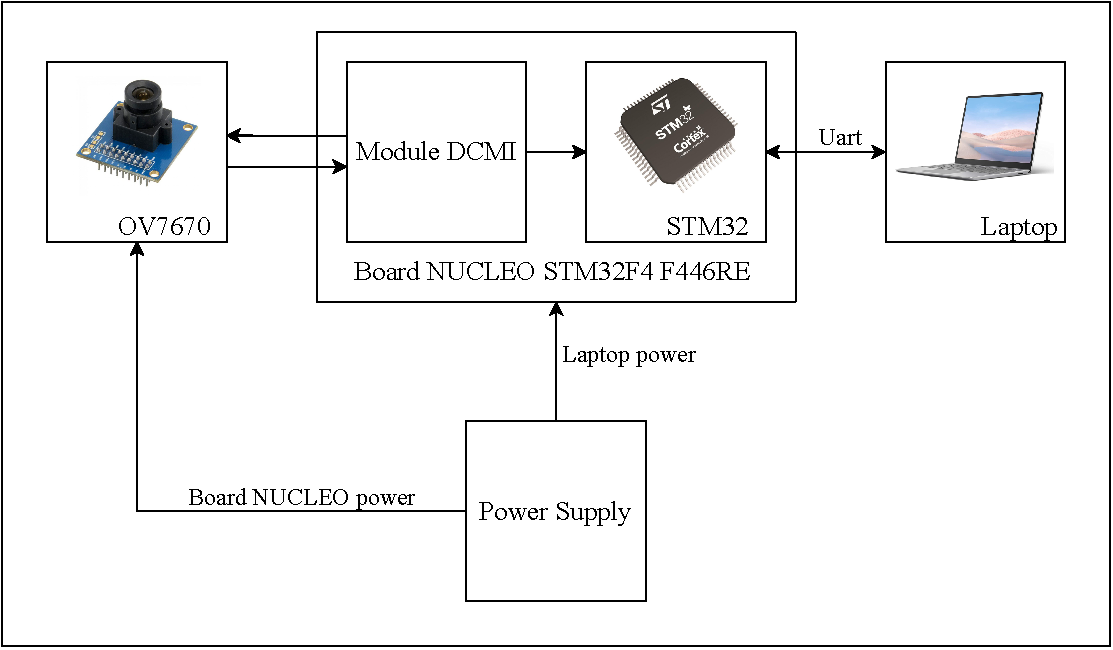
\includegraphics[scale = 0.78]{design_descriptionnew.pdf}
					\caption{\it System Architecture}
				\end{figure}
	\end{otherlanguage}

\end{document}